\cleardoublepage
\phantomsection
\addcontentsline{toc}{chapter}{Nomenklatur}

\chapter*{Nomenklatur}

\begin{longtable}{cp{3cm}p{8cm}}
\hline
Symbol       & Einheit & Beschreibung \\
\hline\hline
$\omega$     & $1/s$   & Kreisfrequenz\\
$T$          & $s$     & Periode      \\
$S_a$        & $m/s^2$ & Spektralbeschleunigung \\
$m$          & $t$     & Masse        \\
$M$          & $t$     & Massenmatrix \\
$k$          & $kN/m$  & Steifigkeit  \\
$K$          & $kN/m$  & Steifigkeitsmatrix \\
$c$          & $-$     & Dämpfungsbeiwert \\
$C$          & $-$     & Dämpfungsmatrix \\
$E$          & $kN/m^2$& Elastizitätsmodul \\
$I$          & $m^4$   & Flächenmoment 2. Grades \\
$F$          & $kN$    & Kraft        \\
$t$          & $s$     & Zeit         \\
$u$          & $m$     & Verschiebung \\
$\xi$        & $-$     & Dämpfung     \\
$\eta$       & $-$     & Dämpfungs-Korrekturbeiwert \\
$a$          & $m/s^2$ & Beschleunigung \\
$P$          & $-$     & Wahrscheinlichkeit \\
$\gamma_1$   & $-$     & Bedeutungsbeiwert \\
$G$          & $t, kN$ & Vertikalkraft (Eigengewicht) \\
$D$          & $m$     & Auslenkung \\
$R$          & $m$     & Radius \\
$\theta$     & $^{\circ}$ & Winkel \\
$\mu$        & $-$     & Reibungskoeffizient \\
$\vec{\Phi}$ & $-$     & Eigenvektor \\
$\varphi$       & $-$     & Eigenvektorkomponente \\
$L$          & $-$     & Beteiligunsfaktor \\
$\vec{I}$    & $-$     & Einheitsvektor \\
$VT$         & $-$     & Transmissibilität \\
\hline
\end{longtable}


\cleardoublepage
\phantomsection
\addcontentsline{toc}{chapter}{\listfigurename}
\listoffigures

\cleardoublepage
\phantomsection
\addcontentsline{toc}{chapter}{Bibliographie}
\printbibliography

\cleardoublepage
\phantomsection
\addcontentsline{toc}{chapter}{Eidesstattliche Erklärung}

\chapter*{Eidesstattliche Erklärung}

Hiermit versichere ich, die vorliegende Master Thesis ohne Hilfe Dritter, nur mit den
angegebenen Quellen und Hilfsmitteln, angefertigt zu haben. Alle Stellen, die den
Quellen entnommen wurden, sind als solche kenntlich gemacht worden.

\vspace*{\fill}

\begin{tabular}{@{}p{.5in}p{4in}@{}}
& \hrulefill \\
& \GetAuthor \\
& \date{\today{}, Karlsruhe}\\
\end{tabular}

\vspace*{\fill}

\cleardoublepage
\phantomsection
\addcontentsline{toc}{chapter}{Datenträger}

\cleardoublepage
\phantomsection
\addcontentsline{toc}{chapter}{Berechnungsprotokoll Modalanalyse mit RStab}
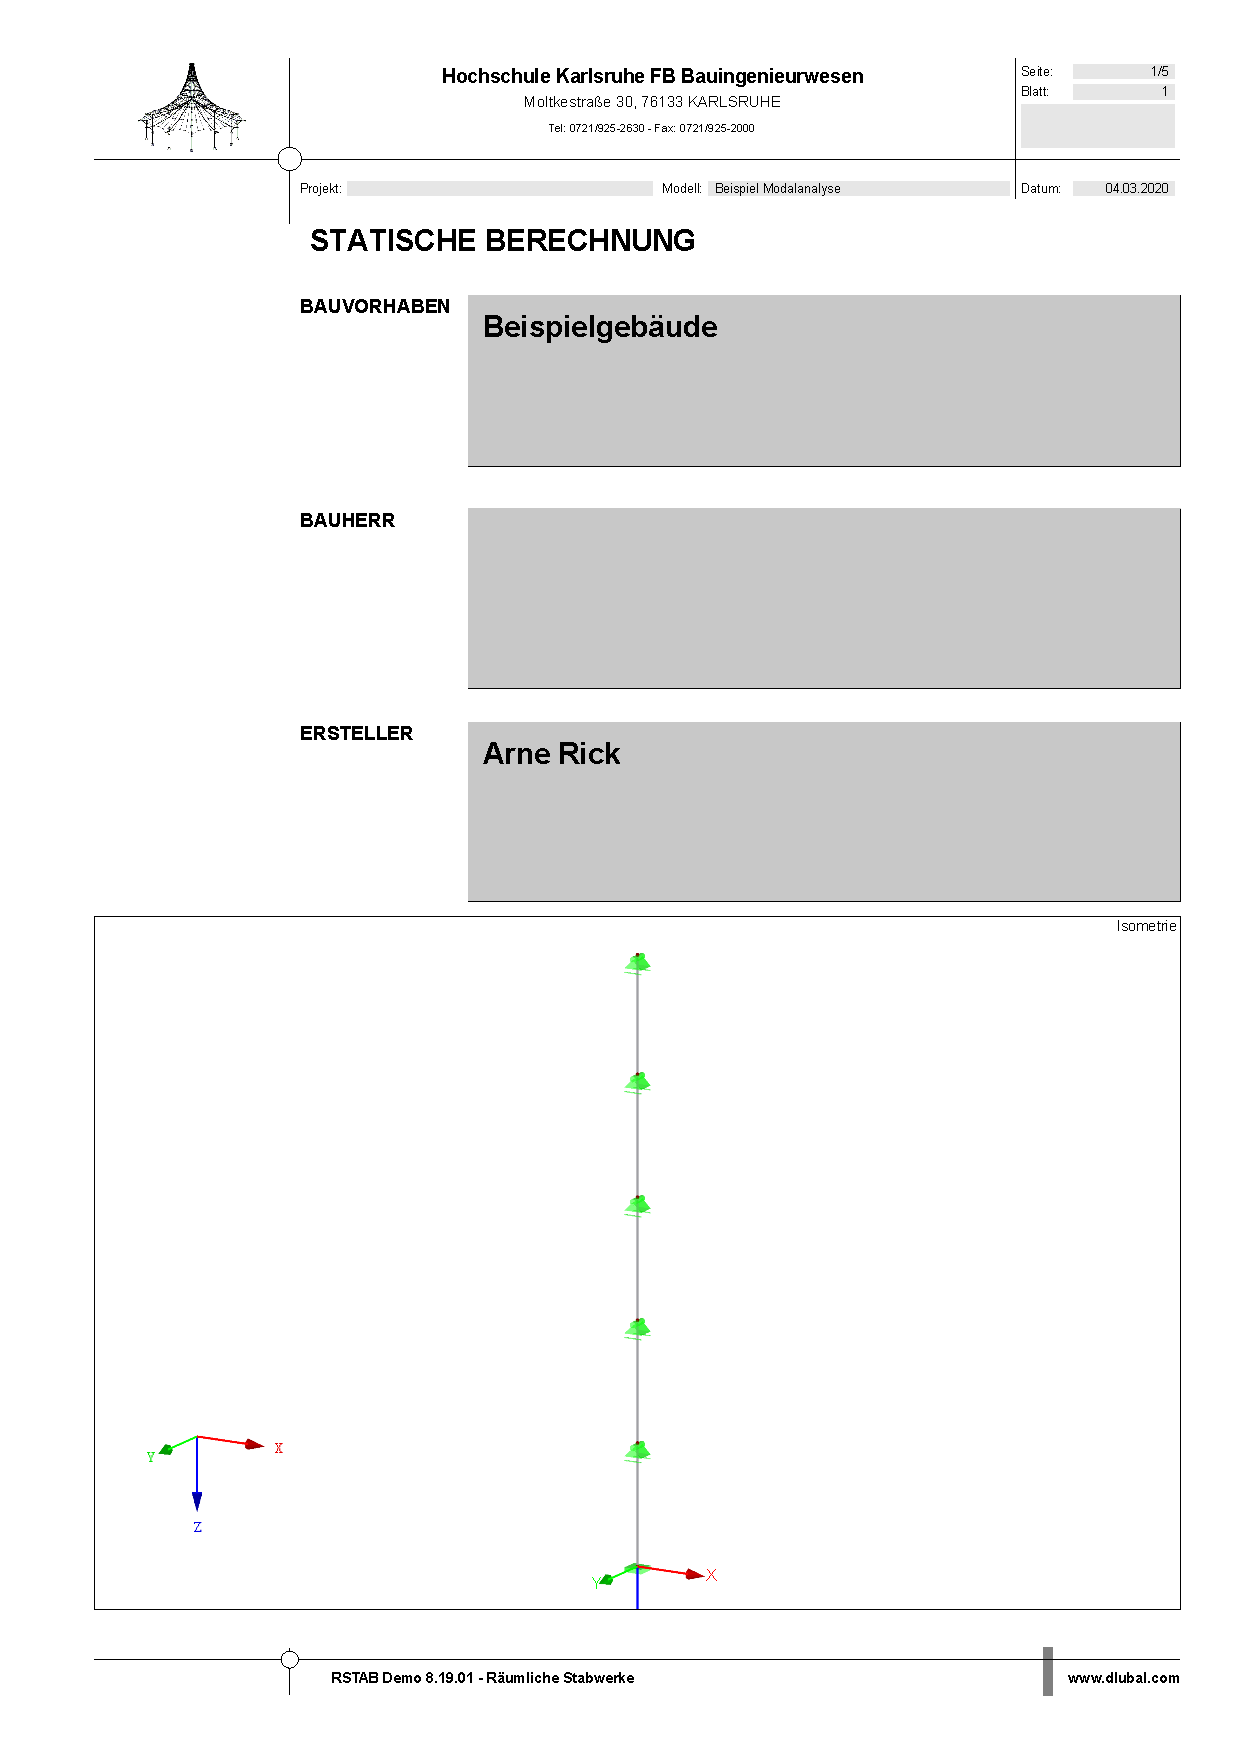
\includepdf[pages=-]{Ausdruckprotokoll_-_RStab.pdf}


